\documentclass[a4paper,12pt]{article}
\usepackage{bbding,combelow,textcomp,amsfonts,amsthm,amsmath,amssymb,graphicx,color,hyperref,etoolbox}
\usepackage[utf8x]{inputenc}
\usepackage[lined,boxed,commentsnumbered]{algorithm2e}
\usepackage{tikz}
\usetikzlibrary{calc,decorations.pathreplacing}

\newtoggle{story}


%%%%%%%%%%%%%%%%%%%%%%%%%%%%%%%%%%%%%%%%%%
%% Customisation options --- update as necessary
%%%%%%%%%%%%%%%%%%%%%%%%%%%%%%%%%%%%%%%%%%

%% Course details: title, semester, instructors

\newcommand{\courseTitle}{Probabilistic Combinatorics (Math 5390)}
\newcommand{\semester}{Fall 2026}
\newcommand{\instructorA}{Shagnik Das}
\newcommand{\instructorB}{}

%% Sheet number

\newcommand{\sheetNumber}{2}


%% Submission details

\newcommand{\dueDate}{12:20, Oct 23rd.}
\newcommand{\lateWarning}{Late submissions will receive no credit.}


%% Display irrelevant footnotes?  \toggletrue for yes, \togglefalse for no

\toggletrue{story}

%%%%%%%%%%%%%%%%%%%%%%%%%%%%%%%%%%%%%%%%%%
%% End of customisation options
%%%%%%%%%%%%%%%%%%%%%%%%%%%%%%%%%%%%%%%%%%

\pdfpagewidth 8.5in
\pdfpageheight 11in
\topmargin -1in
\headheight 0in
\headsep 0in
\textheight 8.5in
\textwidth 6.5in
\oddsidemargin 0in
\evensidemargin 0in
\headheight 77pt
\headsep 0in
\footskip .75in

\makeatletter
\newcommand{\buildtitle}[4]{
\begin{flushleft}
{\large
#1
\hfill{}
#2
\par
#3
}
\end{flushleft}
\vskip 4pt
\begin{center}
{\large\bfseries#4\par}
\end{center}
\bigskip
}
\makeatother

\renewcommand{\thesection}{\normalsize\arabic{section}}

\renewcommand{\deg}{\textrm{deg}}
\newcommand{\eps}{\varepsilon}
\newcommand{\ceil}[1]{\left \lceil #1 \right \rceil}

\newcommand{\hint}{\begin{flushright} [Hint at \url{\hintURL}.] \end{flushright}}

\newcommand{\card}[1]{\left| #1 \right|}
\newcommand{\mb}[1]{\mathbb{#1}}
\newcommand{\mc}[1]{\mathcal{#1}}


\newcommand{\story}[1]{\iftoggle{story}{\footnote{#1}}{}}
\newcommand{\storymark}[1][42]{\iftoggle{story}{\footnotemark[#1]}{}}
\newcommand{\storytext}[2][42]{\iftoggle{story}{\footnotetext[#1]{#2}}{}}

\newcommand{\bonus}[2]{\paragraph{Bonus (#1 pt\ifstrequal{#1}{1}{}{s})} #2}


\begin{document}


\buildtitle{\courseTitle{}}{\semester}{\instructorA{} \hfill \instructorB{}}{Exercise Sheet \sheetNumber{}}

\vspace{-0.2in}

\begin{center}

{\bf Due date: \dueDate \\ \lateWarning}

\end{center}

\noindent You and your partner should try to solve all of the exercises below, and then submit a total of two solutions to be graded --- each problem is worth $10$ points. Both partners should author one solution each, making clear who wrote which solution, but you will earn credit for both solutions. Make sure to clearly justify your answers, defining everything precisely and stating any results you are using. You should then submit your solutions on NTU COOL, either as a typed PDF or a clear picture or scan of your handwritten answers.

\paragraph{Exercise 1}  Given natural numbers $a_1, a_2, \hdots, a_r$ and $b_1, b_2, \hdots, b_s$, we denote by $\mc L$ the linear equation $\sum_{i=1}^r a_i x_i = \sum_{j=1}^s b_j y_j$, and say a set of integers $A$ is \emph{${\mc L}$-free} if it does not contain any solution $(x_1, \hdots, x_r, y_1, \hdots, y_s) \in A^{r+s}$ to $\mc L$. Prove that if $\sum_{i=1}^r a_i \neq \sum_{j=1}^s b_j$, then there is some constant $c = c_{\mc L}$ such that every set $S$ of $n$ non-zero integers contains an $\mc L$-free subset $A \subseteq S$ of size $\card{A} \ge cn$.

\paragraph{Solution.} Write $\sigma_a = \sum_{i=1}^r a_i$ and $\sigma_b = \sum_{j=1}^s b_j$. A set contains a solution to $\mc L$ if and only if it contains a solution to the equation obtained by swapping the two sides of $\mc L$, so we may assume $\sigma_a > \sigma_b$; as these are integers, $\sigma_a - \sigma_b \ge 1$. For $u \in \mb R$ let $\{u\} = u - \lfloor u \rfloor \in [0,1)$ denote its fractional part. Set
\[
	t = \frac{1}{2(\sigma_a - \sigma_b)}, \qquad \delta = \frac{1}{4(\sigma_a + \sigma_b)}, \qquad I = [t - \delta, t + \delta), \qquad c = 2\delta = \frac{1}{2(\sigma_a + \sigma_b)}.
\]
Since $0 < \sigma_a - \sigma_b \le \sigma_a + \sigma_b$, we have $t - \delta \ge \frac{1}{2(\sigma_a+\sigma_b)} - \frac{1}{4(\sigma_a+\sigma_b)} > 0$ and $t + \delta \le \frac12 + \frac14 < 1$, so $I \subseteq (0,1)$ is an interval of length $c$. For $\theta \in [0,1)$ let
\[
	A_\theta = \{ x \in S : \{ x \theta \} \in I \}.
\]

\begin{proof}[Claim 1: $A_\theta$ is $\mc L$-free for every $\theta$]
	Suppose $(x_1, \hdots, x_r, y_1, \hdots, y_s) \in A_\theta^{r+s}$ solves $\mc L$, and put $u = \sum_{i} a_i \{x_i \theta\}$ and $v = \sum_j b_j \{y_j \theta\}$.

	\emph{$u - v$ is an integer.} Each $x_i \theta - \{x_i \theta\}$ and $y_j \theta - \{ y_j \theta \}$ is an integer, and the $a_i, b_j$ are integers, so
	\[
		u - v \equiv \theta \Big( \sum_i a_i x_i - \sum_j b_j y_j \Big) = 0 \pmod 1.
	\]

	\emph{$u - v \in [\frac14, \frac34]$.} Each $\{x_i\theta\}, \{y_j \theta\}$ lies in $[t - \delta, t + \delta]$ and all $a_i, b_j \ge 0$, so $\sigma_a (t - \delta) \le u \le \sigma_a (t + \delta)$ and $\sigma_b (t - \delta) \le v \le \sigma_b (t + \delta)$. Hence
	\[
		u - v \ge (\sigma_a - \sigma_b) t - (\sigma_a + \sigma_b) \delta = \tfrac12 - \tfrac14 = \tfrac14, \qquad u - v \le (\sigma_a - \sigma_b) t + (\sigma_a + \sigma_b) \delta = \tfrac34.
	\]
	As $[\frac14, \frac34]$ contains no integer, this is a contradiction.
\end{proof}

\begin{center}
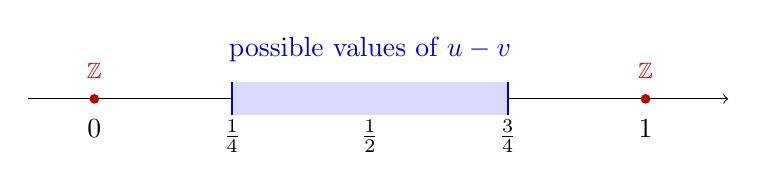
\begin{tikzpicture}[scale=7]
	\draw[->] (-0.12,0) -- (1.15,0);
	\fill[blue!15] (0.25,-0.03) rectangle (0.75,0.03);
	\draw[thick,blue!70!black] (0.25,-0.03) -- (0.25,0.03) (0.75,-0.03) -- (0.75,0.03);
	\foreach \x/\l in {0/0, 0.25/\frac14, 0.5/\frac12, 0.75/\frac34, 1/1} \node[below=4pt] at (\x,0) {$\l$};
	\fill[red!70!black] (0,0) circle (0.25pt) (1,0) circle (0.25pt);
	\node[blue!70!black,above=4pt] at (0.5,0.03) {possible values of $u - v$};
	\node[red!70!black,above=2pt,font=\footnotesize] at (0,0.01) {$\mb Z$};
	\node[red!70!black,above=2pt,font=\footnotesize] at (1,0.01) {$\mb Z$};
\end{tikzpicture}
\end{center}

\begin{proof}[Claim 2: if $\theta$ is uniform on {$[0,1)$} and $x \neq 0$ is an integer, then $\Pr(\{x\theta\} \in I) = c$]
	Let $m = \card{x} \ge 1$ and split $[0,1)$ into the $m$ intervals $J_k = [\frac km, \frac{k+1}{m})$, $0 \le k \le m-1$. On each $J_k$, $x\theta$ runs over an interval of length $1$ between two consecutive integers, so $\theta \mapsto \{x\theta\}$ is an affine map with slope $\pm m$ from $J_k$ onto $[0,1)$ (up to an endpoint). Hence $\{ \theta \in J_k : \{x \theta\} \in I \}$ has length $\card{I} / m = c/m$, and summing over the $m$ intervals gives $\Pr(\{x\theta\} \in I) = c$.
\end{proof}

\begin{proof}[Conclusion]
	Choose $\theta$ uniformly at random from $[0,1)$. Every element of $S$ is a non-zero integer, so by linearity of expectation and Claim 2,
	\[
		\mb E \card{A_\theta} = \sum_{x \in S} \Pr(\{x\theta\} \in I) = cn.
	\]
	Hence some $\theta$ satisfies $\card{A_\theta} \ge cn$, and by Claim 1, $A = A_\theta \subseteq S$ is $\mc L$-free. Thus $c_{\mc L} = \frac{1}{2(\sigma_a + \sigma_b)}$ works.
\end{proof}

\paragraph{Exercise 2}  Recall that a $k$-uniform family of subsets $\mc F \subseteq \binom{[n]}{k}$ is said to be \emph{intersecting} if $F_1 \cap F_2 \neq \emptyset$ for all $F_1, F_2 \in \mc F$. We say that $\mc F$ is \emph{maximally intersecting} if it is intersecting and, if $\mc F \subsetneq \mc F'$, then $\mc F'$ is not intersecting. Given a family $\mc G \subseteq \binom{[n]}{k}$ of sets, we write $\mc I(\mc G) = \left\{ F \in \binom{[n]}{k}: \forall G \in \mc G, \; F \cap G \neq \emptyset \right\}$ for the family of all $k$-sets that intersect every member of $\mc G$. We say a maximally intersecting family $\mc F$ is \emph{generated} by $\mc G$ if $\mc I(\mc G) = \mc F$.

\begin{itemize}
	\item[(a)] Show that $\mc F$ is intersecting if and only if $\mc F \subseteq \mc I( \mc F)$, and it is maximally intersecting if and only if we have equality.
	\item[(b)] Prove that every maximally intersecting family $\mc F$ is generated by a family $\mc G$ with $\card{\mc G} \le \binom{2k}{k}$.
\end{itemize}

\paragraph{Solution (to be graded; provided by Huang).} Throughout $k \ge 1$, so every $F \in \binom{[n]}{k}$ satisfies $F \cap F = F \neq \emptyset$. Note that $\mc I$ is order-reversing: if $\mc G_1 \subseteq \mc G_2$, then $\mc I(\mc G_2) \subseteq \mc I(\mc G_1)$, since a $k$-set meeting every member of $\mc G_2$ in particular meets every member of $\mc G_1$.

\begin{proof}[Proof of (a)]
	By definition, $\mc F \subseteq \mc I(\mc F)$ means that every $F_1 \in \mc F$ meets every $F_2 \in \mc F$, which is exactly the statement that $\mc F$ is intersecting.

	Now suppose $\mc F$ is maximally intersecting; then $\mc F \subseteq \mc I(\mc F)$. If there were some $H \in \mc I(\mc F) \setminus \mc F$, then $\mc F' = \mc F \cup \{H\} \supsetneq \mc F$ would be intersecting: $H$ meets every member of $\mc F$ since $H \in \mc I(\mc F)$, $H \cap H \neq \emptyset$, and any two members of $\mc F$ meet. This contradicts maximality, so $\mc F = \mc I(\mc F)$.

	Conversely, suppose $\mc F = \mc I(\mc F)$. Then $\mc F$ is intersecting by the first part. Let $\mc F' \supsetneq \mc F$ and pick $H \in \mc F' \setminus \mc F$. If $\mc F'$ were intersecting, $H$ would meet every member of $\mc F \subseteq \mc F'$, i.e.\ $H \in \mc I(\mc F) = \mc F$, a contradiction. So $\mc F$ is maximally intersecting.
\end{proof}

We use the following result from lecture.

\medskip
\noindent \textbf{Lemma} (Bollob\'as's set-pairs inequality)\textbf{.} \emph{Let $A_1, \hdots, A_m, B_1, \hdots, B_m \in \binom{[n]}{k}$ satisfy $A_i \cap B_i = \emptyset$ for all $i$, and $A_i \cap B_j \neq \emptyset$ for all $i \neq j$. Then $m \le \binom{2k}{k}$.}

\begin{proof}[Proof of (b)]
	Let $\mc F$ be maximally intersecting. By (a), $\mc I(\mc F) = \mc F$, so $\mc F$ is generated by the subfamily $\mc F$ of itself. Among all subfamilies $\mc G \subseteq \mc F$ with $\mc I(\mc G) = \mc F$, choose one of minimum size, say $\mc G = \{G_1, \hdots, G_m\}$. We show $m \le \binom{2k}{k}$; if $m = 0$ there is nothing to prove.

	Fix $i$. By minimality, $\mc I(\mc G \setminus \{G_i\}) \neq \mc F = \mc I(\mc G)$, while $\mc I(\mc G) \subseteq \mc I(\mc G \setminus \{G_i\})$ as $\mc I$ is order-reversing. So there exists
	\[
		H_i \in \mc I(\mc G \setminus \{G_i\}) \setminus \mc I(\mc G).
	\]
	Since $H_i \in \mc I(\mc G \setminus \{G_i\})$, it meets $G_j$ for every $j \neq i$. Since $H_i \notin \mc I(\mc G)$, it is disjoint from some member of $\mc G$, which can only be $G_i$. Thus
	\[
		G_i \cap H_i = \emptyset \quad \text{for all } i, \qquad G_j \cap H_i \neq \emptyset \quad \text{for all } i \neq j.
	\]
	Applying the Lemma with $A_i = G_i$ and $B_i = H_i$ gives $\card{\mc G} = m \le \binom{2k}{k}$, and $\mc G$ generates $\mc F$.
\end{proof}

\paragraph{Exercise 3}  Recall the asymmetric Ramsey number $R(k, \ell)$ is the smallest $n$ such that every red-/blue-edge-colouring of $K_n$ contains a red $K_k$ or a blue $K_{\ell}$.
\begin{itemize}
	\item[(a)] Show that for any integer $n$ and $p \in [0,1]$, we have
\[ R(k, \ell) > n - \binom{n}{k} p^{\binom{k}{2}} - \binom{n}{\ell} (1 - p)^{\binom{\ell}{2}}. \]
	\item[(b)] Use the result from (a) to prove the best lower bound on $R(3, \ell)$ (as $\ell \to \infty$) that you can.
\end{itemize}

\paragraph{Solution.} Throughout, $\ln$ is the natural logarithm and $k, \ell \ge 1$.

\begin{proof}[Proof of (a)]
	If $n \le 0$, the right-hand side is at most $n \le 0 < R(k, \ell)$, so assume $n \ge 1$. Colour each edge of $K_n$ red with probability $p$ and blue otherwise, independently. Let $X$ be the number of red copies of $K_k$ and $Y$ the number of blue copies of $K_\ell$. A fixed $k$-set of vertices spans a red $K_k$ exactly when all of its $\binom k2$ edges are red, so by linearity of expectation
	\[
		\mb E[X + Y] = \binom nk p^{\binom k2} + \binom n\ell (1-p)^{\binom \ell2}.
	\]
	Hence there is a colouring with $X + Y \le \mb E[X+Y]$. Fix such a colouring, and delete one vertex from each red $K_k$ and each blue $K_\ell$. This leaves a set $W$ of $m \ge n - X - Y \ge n - \mb E[X + Y]$ vertices, and the colouring on $W$ has no red $K_k$ and no blue $K_\ell$, since each such copy lost a vertex. Restricting to any $m' \le m$ vertices of $W$ gives the same property, so no $n' \le m$ satisfies the defining property of $R(k, \ell)$. Thus
	\[
		R(k, \ell) > m \ge n - \binom nk p^{\binom k2} - \binom n\ell (1-p)^{\binom \ell2}. \qedhere
	\]
\end{proof}

\begin{proof}[Proof of (b)]
	We show $R(3, \ell) = \Omega\big( (\ell / \ln \ell)^{3/2} \big)$. Fix $p \in (0,1]$. Using $\binom n3 \le \frac{n^3}{6}$, $\binom n\ell \le \left( \frac{en}{\ell} \right)^\ell$ and $1 - p \le e^{-p}$, (a) gives for every $n$
	\begin{equation}
		R(3, \ell) > \underbrace{n - \frac{p^3 n^3}{6}}_{=: h(n)} - \Big( \underbrace{\frac{en}{\ell} e^{-p(\ell-1)/2}}_{=: b(n,p)} \Big)^\ell. \label{eq:R3} \tag{$\star$}
	\end{equation}

	\emph{Step 1: choosing $n$ in terms of $p$.} Since $h'(x) = 1 - \frac{p^3 x^2}{2}$, $h$ increases on $[0, x^*]$ and decreases afterwards, where $x^* = \sqrt 2 \, p^{-3/2}$ solves $h'(x^*) = 0$; so the best choice is $n \approx x^*$. Take $n = \lfloor x^* \rfloor$, so $x^* - 1 < n \le x^*$. From $n \le x^* = \sqrt 2 \, p^{-3/2}$ we get $p^3 n^2 \le 2$, hence
	\[
		h(n) = n \left( 1 - \frac{p^3 n^2}{6} \right) \ge n \left( 1 - \frac{2}{6} \right) = \frac{2n}{3} > \frac23 (x^* - 1) = \frac{2\sqrt 2}{3} p^{-3/2} - \frac23.
	\]

	\emph{Step 2: choosing $p$.} By Step 1, the main term of \eqref{eq:R3} is $F(p) = \frac{2\sqrt 2}{3} p^{-3/2}$, and $F'(p) = -\sqrt 2 \, p^{-5/2} < 0$, so we want $p$ as small as possible. The only constraint is that the blue term should be negligible, i.e.\ $b(n,p)^\ell = o(1)$ as $\ell \to \infty$. Try $p = \frac{c \ln \ell}{\ell - 1}$ with $c > 0$. Then $e^{-p(\ell-1)/2} = \ell^{-c/2}$ and $p^{-1} = \frac{\ell - 1}{c \ln \ell} \le \frac{\ell}{c \ln \ell}$ (as $\ell - 1 \le \ell$), so using $n \le \sqrt 2 \, p^{-3/2}$,
	\[
		b(n,p) \le \frac{e \sqrt 2}{\ell} \left( \frac{\ell}{c \ln \ell} \right)^{3/2} \ell^{-c/2} = \frac{e \sqrt 2}{c^{3/2}} \cdot \frac{\ell^{(1-c)/2}}{(\ln \ell)^{3/2}}.
	\]
	This tends to $0$ exactly when $c \ge 1$, and then $b(n,p)^\ell \le b(n,p) = o(1)$. As $F$ is decreasing, we take the smallest such value $c = 1$, i.e.
	\[
		p = \frac{\ln \ell}{\ell - 1} \in (0, 1], \qquad b(n,p) \le \frac{e \sqrt 2}{(\ln \ell)^{3/2}}.
	\]

	\emph{Conclusion.} For $\ell \ge 12$ we have $(\ln \ell)^{3/2} > e \sqrt 2$, so $b(n,p) < 1$ and $b(n,p)^\ell \le b(n,p) = o(1)$. By \eqref{eq:R3} and Step 1,
	\[
		R(3, \ell) > \frac{2 \sqrt 2}{3} p^{-3/2} - \frac23 - o(1) = \frac{2 \sqrt 2}{3} \left( \frac{\ell - 1}{\ln \ell} \right)^{3/2} - O(1) = \Omega\left( \left( \frac{\ell}{\ln \ell} \right)^{3/2} \right).
	\]
	Step 1 shows that (a) never gives more than $O(p^{-3/2})$, and Step 2 that the blue term forces $p = \Omega\left( \frac{\ln \ell}{\ell} \right)$, so this is the best bound obtainable from (a), up to the constant.
\end{proof}

\paragraph{Exercise 4}  In this exercise you will provide an explicit construction of a set of $n$ points in $[0,1]^2$, such that every triple of points determines a triangle of area $\Omega \left( \frac{1}{n^2} \right)$.
\begin{itemize}
	\item[(a)] Let $p$ be prime, and let $S = \{ (x, x^2 \pmod{p} ) : 0 \le x \le p-1 \}$. Prove that there are no three points of $S$ lying on a common line.
	\item[(b)] By rescaling $S$ appropriately, show that we can find $p$ points in $[0,1]^2$, such that every triangle has area at least $\frac{1}{2(p-1)^2}$.
	\item[(c)] Deduce the existence of the desired set of points for all $n \ge 2$.
\end{itemize}

\paragraph{Solution (to be graded; provided by Chang).} Throughout, $x^2 \pmod p$ denotes the representative in $\{0, 1, \hdots, p-1\}$, so $S \subseteq \{0, 1, \hdots, p-1\}^2 \subseteq \mb Z^2$. For points $P_i = (x_i, y_i) \in \mb R^2$, $i = 1, 2, 3$, write
\[
	D(P_1, P_2, P_3) = \det \begin{pmatrix} 1 & x_1 & y_1 \\ 1 & x_2 & y_2 \\ 1 & x_3 & y_3 \end{pmatrix}.
\]
Recall that the triangle $P_1 P_2 P_3$ has area $\frac12 \card{D(P_1, P_2, P_3)}$, and in particular $P_1, P_2, P_3$ are collinear if and only if $D(P_1, P_2, P_3) = 0$.

\begin{proof}[Proof of (a)]
	Take three distinct points of $S$. Each has the form $P_i = (x_i, y_i)$ with $x_i \in \{0, 1, \hdots, p-1\}$ and $y_i = x_i^2 \pmod p$, for $i = 1, 2, 3$. If $x_i = x_j$, then also $y_i = y_j$, so $P_i = P_j$; hence $x_1, x_2, x_3$ are pairwise distinct. It suffices to show that $D = D(P_1, P_2, P_3) \neq 0$.

	Since $y_i$ is the remainder of $x_i^2$ upon division by $p$, there are integers $q_i$ with $y_i = x_i^2 - p q_i$ for $i = 1, 2, 3$. Thus the third column of the matrix defining $D$ is $(x_i^2)_i - p\,(q_i)_i$, and since the determinant is linear in its third column,
	\[
		D = \underbrace{\det \begin{pmatrix} 1 & x_1 & x_1^2 \\ 1 & x_2 & x_2^2 \\ 1 & x_3 & x_3^2 \end{pmatrix}}_{=: V} - \, p \underbrace{\det \begin{pmatrix} 1 & x_1 & q_1 \\ 1 & x_2 & q_2 \\ 1 & x_3 & q_3 \end{pmatrix}}_{=: E}.
	\]
	Both $V$ and $E$ are determinants of integer matrices, hence integers, so $D \equiv V \pmod p$. Moreover $V$ is a Vandermonde determinant, so
	\[
		V = (x_2 - x_1)(x_3 - x_1)(x_3 - x_2).
	\]
	As $0 \le x_i \le p-1$ are distinct, each difference $x_j - x_i$ satisfies $0 < \card{x_j - x_i} < p$, so is not divisible by $p$. Since $p$ is prime, the product $V$ is not divisible by $p$ either. Hence $D \equiv V \not\equiv 0 \pmod p$; in particular $D \neq 0$, and $P_1, P_2, P_3$ are not collinear.
\end{proof}

\begin{proof}[Proof of (b)]
	For $p = 2$ there are no triangles, so assume $p \ge 3$. Let $S' = \frac{1}{p-1} S = \left\{ \left( \frac{x}{p-1}, \frac{x^2 \pmod p}{p-1} \right) : 0 \le x \le p-1 \right\}$. Since all coordinates of points of $S$ lie in $\{0, \hdots, p-1\}$, we have $S' \subseteq [0,1]^2$, and $\card{S'} = \card{S} = p$.

	Take three distinct points of $S'$; they are $\frac{1}{p-1} P_1, \frac{1}{p-1} P_2, \frac{1}{p-1} P_3$ for distinct $P_1, P_2, P_3 \in S$. Let $D = D(P_1, P_2, P_3)$. We claim $\card{D} \ge 1$:
	\begin{itemize}
		\item $D \in \mb Z$: every entry of the matrix defining $D$ is an integer (the coordinates of points of $S$ are integers), and a determinant is a sum of products of entries with signs $\pm 1$, so it is an integer.
		\item $D \neq 0$: this was shown in the proof of (a).
	\end{itemize}
	A non-zero integer has absolute value at least $1$, so $\card{D} \ge 1$, and the triangle $P_1 P_2 P_3$ has area $\frac12 \card{D} \ge \frac12$.

	Finally, multiplying the second and third columns of the matrix by $\frac{1}{p-1}$ multiplies the determinant by $\frac{1}{(p-1)^2}$, so
	\[
		D\left( \tfrac{1}{p-1} P_1, \tfrac{1}{p-1} P_2, \tfrac{1}{p-1} P_3 \right) = \frac{D}{(p-1)^2},
	\]
	and the triangle with vertices $\frac{1}{p-1} P_i$ has area $\frac{\card{D}}{2(p-1)^2} \ge \frac{1}{2(p-1)^2}$.
\end{proof}

\begin{proof}[Proof of (c)]
	If $n = 2$, any two distinct points of $[0,1]^2$ work: there is no triple of points, hence no triangle, so there is nothing to check. Now let $n \ge 3$. By Bertrand's postulate (for every integer $m > 1$ there is a prime $p$ with $m < p < 2m$), there is a prime $p$ with $n < p < 2n$. Let $T$ be any $n$ points of the set $S'$ from (b). Then $T \subseteq [0,1]^2$, and every triangle with vertices in $T$ is a triangle with vertices in $S'$, so its area is at least
	\[
		\frac{1}{2(p-1)^2} > \frac{1}{2(2n)^2} = \frac{1}{8n^2}.
	\]
	Hence every triple of points of $T$ determines a triangle of area $\Omega\left( \frac{1}{n^2} \right)$.
\end{proof}

%\newpage

%\section*{Hints}  The following QR codes contain hints for some of the homework exercises.  You should be able to decode them using any QR code scanner, including this one: \url{https://zxing.org/w/decode.jspx}.

%\paragraph{Exercise 2} Also available at \url{https://i.ibb.co/nqSqFhrY/S02E2.png}.

%\begin{center}
%	\includegraphics[scale=0.5]{Hints/S02E2.png}
%\end{center}

%\paragraph{Exercise 4} Also available at \url{https://i.ibb.co/8g54cRk3/S02E4.png}.

%\begin{center}
%	\includegraphics[scale=0.5]{Hints/S02E4.png}
%\end{center}

\end{document}